\documentclass{standalone}
\usepackage{tikz}
\usetikzlibrary{patterns, positioning}
\usepackage[sfdefault]{ClearSans} %% option 'sfdefault' activates Clear Sans as the default text font
\usepackage[T1]{fontenc}

\begin{document}
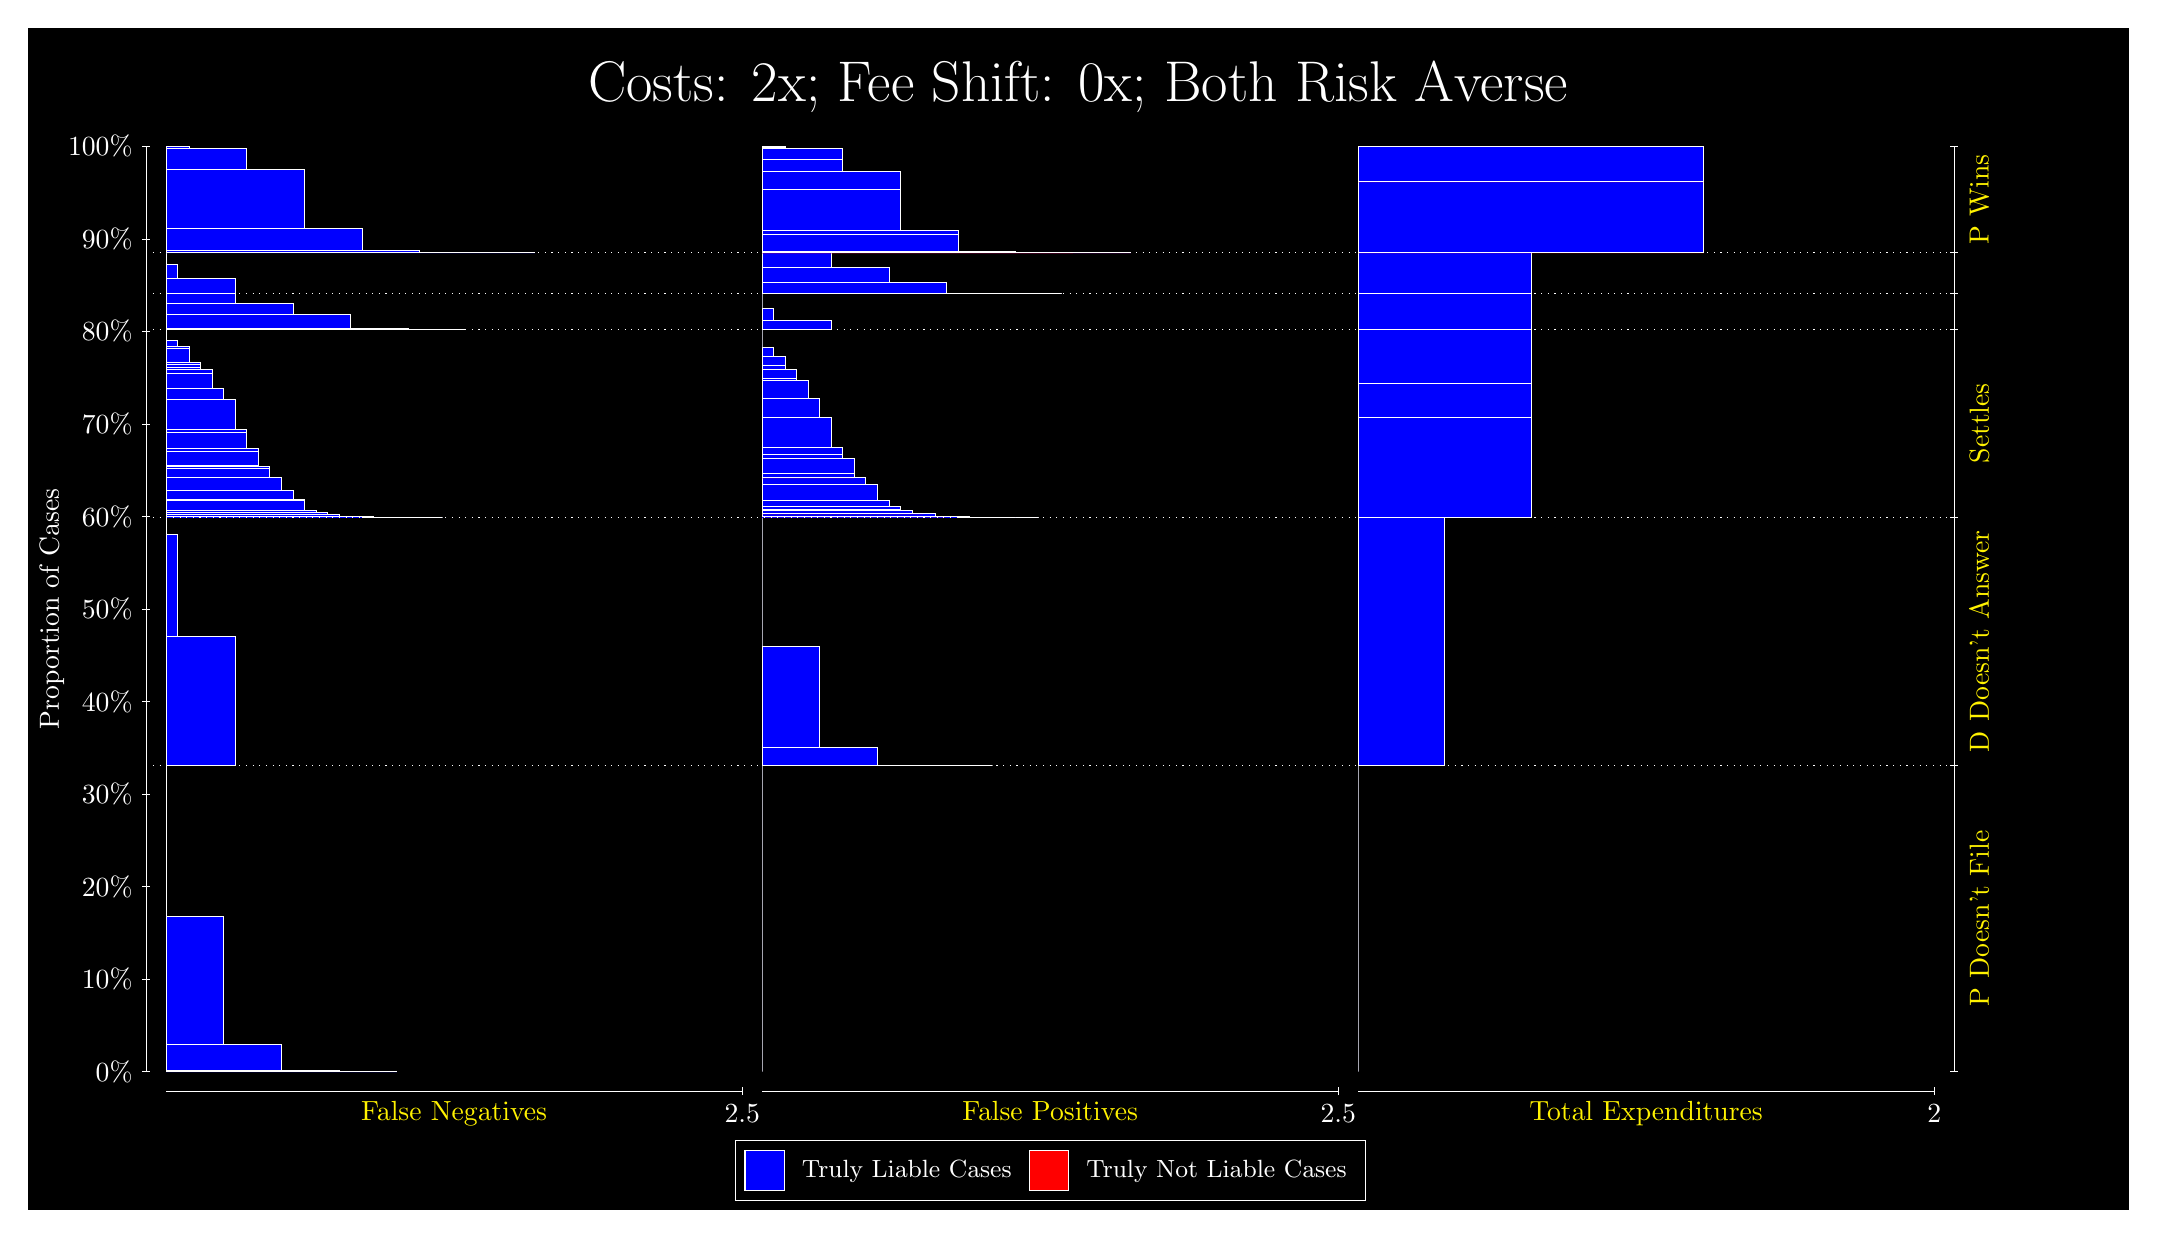
\begin{tikzpicture}
\draw[fill=black] (0,0) rectangle (26.667,15);
\draw[text=white] (0,13.5) rectangle (26.667,15) node[midway] {\huge Costs: 2x; Fee Shift: 0x; Both Risk Averse};
\draw[white, very thin] (1.5,1.75) -- (1.5,13.5);
\node[rotate=90, text=white, anchor=center] at (0.3, 7.625) {Proportion of Cases};
\draw[white, very thin] (1.45,1.75) -- (1.55,1.75);
\node[text=white, anchor=east] at (1.45, 1.75) {0\%};
\draw[white, very thin] (1.45,2.925) -- (1.55,2.925);
\node[text=white, anchor=east] at (1.45, 2.925) {10\%};
\draw[white, very thin] (1.45,4.1) -- (1.55,4.1);
\node[text=white, anchor=east] at (1.45, 4.1) {20\%};
\draw[white, very thin] (1.45,5.275) -- (1.55,5.275);
\node[text=white, anchor=east] at (1.45, 5.275) {30\%};
\draw[white, very thin] (1.45,6.45) -- (1.55,6.45);
\node[text=white, anchor=east] at (1.45, 6.45) {40\%};
\draw[white, very thin] (1.45,7.625) -- (1.55,7.625);
\node[text=white, anchor=east] at (1.45, 7.625) {50\%};
\draw[white, very thin] (1.45,8.8) -- (1.55,8.8);
\node[text=white, anchor=east] at (1.45, 8.8) {60\%};
\draw[white, very thin] (1.45,9.975) -- (1.55,9.975);
\node[text=white, anchor=east] at (1.45, 9.975) {70\%};
\draw[white, very thin] (1.45,11.15) -- (1.55,11.15);
\node[text=white, anchor=east] at (1.45, 11.15) {80\%};
\draw[white, very thin] (1.45,12.325) -- (1.55,12.325);
\node[text=white, anchor=east] at (1.45, 12.325) {90\%};
\draw[white, very thin] (1.45,13.5) -- (1.55,13.5);
\node[text=white, anchor=east] at (1.45, 13.5) {100\%};

\draw[white, very thin] (24.457,1.75) -- (24.457,13.5);
\draw[white, very thin] (24.407,1.75) -- (24.507,1.75);
\node[anchor=west] at (24.407, 1.75) {};
\draw[white, very thin] (24.407,5.6405) -- (24.507,5.6405);
\node[anchor=west] at (24.407, 5.6405) {};
\draw[white, very thin] (24.407,8.7916) -- (24.507,8.7916);
\node[anchor=west] at (24.407, 8.7916) {};
\draw[white, very thin] (24.407,11.174) -- (24.507,11.174);
\node[anchor=west] at (24.407, 11.174) {};
\draw[white, very thin] (24.407,11.631) -- (24.507,11.631);
\node[anchor=west] at (24.407, 11.631) {};
\draw[white, very thin] (24.407,12.151) -- (24.507,12.151);
\node[anchor=west] at (24.407, 12.151) {};
\draw[white, very thin] (24.407,13.5) -- (24.507,13.5);
\node[anchor=west] at (24.407, 13.5) {};

\draw[white, very thin, fill=blue] (1.75,1.75) rectangle (4.6775,1.7501);
\draw[white, very thin, fill=blue] (1.75,1.7501) rectangle (3.9457,1.7601);
\draw[white, very thin, fill=blue] (1.75,1.7601) rectangle (3.2138,2.0973);
\draw[white, very thin, fill=blue] (1.75,2.0973) rectangle (2.4819,3.7215);
\draw[white, very thin, fill=red] (1.75,3.7215) rectangle (1.75,3.7215);
\draw[white, very thin, fill=blue] (1.75,3.7215) rectangle (1.75,5.6405);
\draw[white, very thin, fill=blue] (1.75,5.6405) rectangle (2.6283,7.2823);
\draw[white, very thin, fill=blue] (1.75,7.2823) rectangle (1.8964,8.5691);
\draw[white, very thin, fill=red] (1.75,8.5691) rectangle (1.75,8.5691);
\draw[white, very thin, fill=blue] (1.75,8.5691) rectangle (1.75,8.7916);
\draw[white, very thin, fill=blue] (1.75,8.7916) rectangle (5.2631,8.7916);
\draw[white, very thin, fill=blue] (1.75,8.7916) rectangle (4.9703,8.7916);
\draw[white, very thin, fill=blue] (1.75,8.7916) rectangle (4.6775,8.7934);
\draw[white, very thin, fill=blue] (1.75,8.7934) rectangle (4.5312,8.7943);
\draw[white, very thin, fill=blue] (1.75,8.7943) rectangle (4.3848,8.7943);
\draw[white, very thin, fill=blue] (1.75,8.7943) rectangle (4.3848,8.7962);
\draw[white, very thin, fill=blue] (1.75,8.7962) rectangle (4.2384,8.7973);
\draw[white, very thin, fill=blue] (1.75,8.7973) rectangle (4.092,8.8079);
\draw[white, very thin, fill=blue] (1.75,8.8079) rectangle (3.9457,8.8257);
\draw[white, very thin, fill=blue] (1.75,8.8257) rectangle (3.7993,8.8472);
\draw[white, very thin, fill=blue] (1.75,8.8472) rectangle (3.6529,8.8497);
\draw[white, very thin, fill=blue] (1.75,8.8497) rectangle (3.6529,8.8772);
\draw[white, very thin, fill=blue] (1.75,8.8772) rectangle (3.5065,9.0072);
\draw[white, very thin, fill=blue] (1.75,9.0072) rectangle (3.5065,9.0216);
\draw[white, very thin, fill=blue] (1.75,9.0216) rectangle (3.3602,9.1326);
\draw[white, very thin, fill=blue] (1.75,9.1326) rectangle (3.2138,9.3016);
\draw[white, very thin, fill=blue] (1.75,9.3016) rectangle (3.0674,9.4107);
\draw[white, very thin, fill=blue] (1.75,9.4107) rectangle (3.0674,9.4308);
\draw[white, very thin, fill=blue] (1.75,9.4308) rectangle (2.921,9.4517);
\draw[white, very thin, fill=blue] (1.75,9.4517) rectangle (2.921,9.6216);
\draw[white, very thin, fill=blue] (1.75,9.6216) rectangle (2.921,9.6702);
\draw[white, very thin, fill=blue] (1.75,9.6702) rectangle (2.7746,9.8736);
\draw[white, very thin, fill=blue] (1.75,9.8736) rectangle (2.7746,9.9019);
\draw[white, very thin, fill=blue] (1.75,9.9019) rectangle (2.6283,10.285);
\draw[white, very thin, fill=blue] (1.75,10.285) rectangle (2.4819,10.426);
\draw[white, very thin, fill=blue] (1.75,10.426) rectangle (2.3355,10.62);
\draw[white, very thin, fill=blue] (1.75,10.62) rectangle (2.3355,10.674);
\draw[white, very thin, fill=blue] (1.75,10.674) rectangle (2.1891,10.688);
\draw[white, very thin, fill=blue] (1.75,10.688) rectangle (2.1891,10.734);
\draw[white, very thin, fill=blue] (1.75,10.734) rectangle (2.1891,10.752);
\draw[white, very thin, fill=blue] (1.75,10.752) rectangle (2.0428,10.938);
\draw[white, very thin, fill=blue] (1.75,10.938) rectangle (2.0428,10.957);
\draw[white, very thin, fill=blue] (1.75,10.957) rectangle (1.8964,11.038);
\draw[white, very thin, fill=red] (1.75,11.038) rectangle (1.75,11.038);
\draw[white, very thin, fill=blue] (1.75,11.038) rectangle (1.75,11.174);
\draw[white, very thin, fill=blue] (1.75,11.174) rectangle (5.5558,11.174);
\draw[white, very thin, fill=blue] (1.75,11.174) rectangle (4.8239,11.189);
\draw[white, very thin, fill=blue] (1.75,11.189) rectangle (4.092,11.361);
\draw[white, very thin, fill=blue] (1.75,11.361) rectangle (3.3602,11.508);
\draw[white, very thin, fill=blue] (1.75,11.508) rectangle (2.6283,11.631);
\draw[white, very thin, fill=red] (1.75,11.631) rectangle (1.75,11.631);
\draw[white, very thin, fill=blue] (1.75,11.631) rectangle (2.6283,11.823);
\draw[white, very thin, fill=blue] (1.75,11.823) rectangle (1.8964,12.006);
\draw[white, very thin, fill=red] (1.75,12.006) rectangle (1.75,12.006);
\draw[white, very thin, fill=blue] (1.75,12.006) rectangle (1.75,12.151);
\draw[white, very thin, fill=blue] (1.75,12.151) rectangle (6.4341,12.151);
\draw[white, very thin, fill=blue] (1.75,12.151) rectangle (5.7022,12.152);
\draw[white, very thin, fill=blue] (1.75,12.152) rectangle (4.9703,12.175);
\draw[white, very thin, fill=blue] (1.75,12.175) rectangle (4.2384,12.465);
\draw[white, very thin, fill=blue] (1.75,12.465) rectangle (3.5065,13.211);
\draw[white, very thin, fill=blue] (1.75,13.211) rectangle (2.7746,13.481);
\draw[white, very thin, fill=blue] (1.75,13.481) rectangle (2.0428,13.5);
\draw[white, very thin, fill=red] (1.75,13.5) rectangle (1.75,13.5);
\draw[white, very thin, fill=blue] (1.75,13.5) rectangle (1.75,13.5);
\draw[white, very thin, fill=red] (9.3189,1.75) rectangle (9.3189,1.75);
\draw[white, very thin, fill=blue] (9.3189,1.75) rectangle (9.3189,5.6405);
\draw[white, very thin, fill=red] (9.3189,5.6405) rectangle (12.246,5.6405);
\draw[white, very thin, fill=blue] (9.3189,5.6405) rectangle (12.246,5.6405);
\draw[white, very thin, fill=blue] (9.3189,5.6405) rectangle (11.515,5.6425);
\draw[white, very thin, fill=blue] (9.3189,5.6425) rectangle (10.783,5.863);
\draw[white, very thin, fill=blue] (9.3189,5.863) rectangle (10.051,7.1498);
\draw[white, very thin, fill=blue] (9.3189,7.1498) rectangle (9.3189,8.7916);
\draw[white, very thin, fill=red] (9.3189,8.7916) rectangle (12.832,8.7916);
\draw[white, very thin, fill=blue] (9.3189,8.7916) rectangle (12.832,8.7916);
\draw[white, very thin, fill=red] (9.3189,8.7916) rectangle (12.539,8.7916);
\draw[white, very thin, fill=blue] (9.3189,8.7916) rectangle (12.539,8.7916);
\draw[white, very thin, fill=red] (9.3189,8.7916) rectangle (12.246,8.7916);
\draw[white, very thin, fill=blue] (9.3189,8.7916) rectangle (12.246,8.7942);
\draw[white, very thin, fill=blue] (9.3189,8.7942) rectangle (12.1,8.7944);
\draw[white, very thin, fill=red] (9.3189,8.7944) rectangle (11.954,8.7944);
\draw[white, very thin, fill=blue] (9.3189,8.7944) rectangle (11.954,8.797);
\draw[white, very thin, fill=blue] (9.3189,8.797) rectangle (11.807,8.7976);
\draw[white, very thin, fill=red] (9.3189,8.7976) rectangle (11.661,8.7976);
\draw[white, very thin, fill=blue] (9.3189,8.7976) rectangle (11.661,8.8051);
\draw[white, very thin, fill=blue] (9.3189,8.8051) rectangle (11.515,8.8352);
\draw[white, very thin, fill=red] (9.3189,8.8352) rectangle (11.368,8.8352);
\draw[white, very thin, fill=blue] (9.3189,8.8352) rectangle (11.368,8.8451);
\draw[white, very thin, fill=blue] (9.3189,8.8451) rectangle (11.222,8.8801);
\draw[white, very thin, fill=blue] (9.3189,8.8801) rectangle (11.075,8.8948);
\draw[white, very thin, fill=red] (9.3189,8.8948) rectangle (11.075,8.8948);
\draw[white, very thin, fill=blue] (9.3189,8.8948) rectangle (11.075,8.9279);
\draw[white, very thin, fill=blue] (9.3189,8.9279) rectangle (10.929,9.009);
\draw[white, very thin, fill=red] (9.3189,9.009) rectangle (10.783,9.009);
\draw[white, very thin, fill=blue] (9.3189,9.009) rectangle (10.783,9.213);
\draw[white, very thin, fill=blue] (9.3189,9.213) rectangle (10.636,9.2919);
\draw[white, very thin, fill=red] (9.3189,9.2919) rectangle (10.49,9.2919);
\draw[white, very thin, fill=blue] (9.3189,9.2919) rectangle (10.49,9.3451);
\draw[white, very thin, fill=blue] (9.3189,9.3451) rectangle (10.49,9.5398);
\draw[white, very thin, fill=blue] (9.3189,9.5398) rectangle (10.344,9.5921);
\draw[white, very thin, fill=blue] (9.3189,9.5921) rectangle (10.344,9.6801);
\draw[white, very thin, fill=blue] (9.3189,9.6801) rectangle (10.197,10.064);
\draw[white, very thin, fill=blue] (9.3189,10.064) rectangle (10.051,10.295);
\draw[white, very thin, fill=blue] (9.3189,10.295) rectangle (9.9044,10.535);
\draw[white, very thin, fill=blue] (9.3189,10.535) rectangle (9.758,10.555);
\draw[white, very thin, fill=blue] (9.3189,10.555) rectangle (9.758,10.664);
\draw[white, very thin, fill=blue] (9.3189,10.664) rectangle (9.6116,10.721);
\draw[white, very thin, fill=blue] (9.3189,10.721) rectangle (9.6116,10.833);
\draw[white, very thin, fill=blue] (9.3189,10.833) rectangle (9.4652,10.944);
\draw[white, very thin, fill=blue] (9.3189,10.944) rectangle (9.3189,11.174);
\draw[white, very thin, fill=red] (9.3189,11.174) rectangle (10.197,11.174);
\draw[white, very thin, fill=blue] (9.3189,11.174) rectangle (10.197,11.297);
\draw[white, very thin, fill=blue] (9.3189,11.297) rectangle (9.4652,11.444);
\draw[white, very thin, fill=blue] (9.3189,11.444) rectangle (9.3189,11.631);
\draw[white, very thin, fill=red] (9.3189,11.631) rectangle (13.125,11.631);
\draw[white, very thin, fill=blue] (9.3189,11.631) rectangle (13.125,11.631);
\draw[white, very thin, fill=blue] (9.3189,11.631) rectangle (12.393,11.639);
\draw[white, very thin, fill=blue] (9.3189,11.639) rectangle (11.661,11.776);
\draw[white, very thin, fill=blue] (9.3189,11.776) rectangle (10.929,11.959);
\draw[white, very thin, fill=blue] (9.3189,11.959) rectangle (10.197,12.151);
\draw[white, very thin, fill=red] (9.3189,12.151) rectangle (14.003,12.151);
\draw[white, very thin, fill=blue] (9.3189,12.151) rectangle (14.003,12.151);
\draw[white, very thin, fill=red] (9.3189,12.151) rectangle (13.271,12.151);
\draw[white, very thin, fill=blue] (9.3189,12.151) rectangle (13.271,12.152);
\draw[white, very thin, fill=red] (9.3189,12.152) rectangle (12.539,12.152);
\draw[white, very thin, fill=blue] (9.3189,12.152) rectangle (12.539,12.171);
\draw[white, very thin, fill=blue] (9.3189,12.171) rectangle (11.807,12.384);
\draw[white, very thin, fill=red] (9.3189,12.384) rectangle (11.807,12.384);
\draw[white, very thin, fill=blue] (9.3189,12.384) rectangle (11.807,12.44);
\draw[white, very thin, fill=blue] (9.3189,12.44) rectangle (11.075,12.952);
\draw[white, very thin, fill=red] (9.3189,12.952) rectangle (11.075,12.952);
\draw[white, very thin, fill=blue] (9.3189,12.952) rectangle (11.075,13.186);
\draw[white, very thin, fill=blue] (9.3189,13.186) rectangle (10.344,13.336);
\draw[white, very thin, fill=blue] (9.3189,13.336) rectangle (10.344,13.477);
\draw[white, very thin, fill=blue] (9.3189,13.477) rectangle (9.6116,13.484);
\draw[white, very thin, fill=blue] (9.3189,13.484) rectangle (9.6116,13.5);
\draw[white, very thin, fill=blue] (9.3189,13.5) rectangle (9.3189,13.5);
\draw[white, very thin, fill=red] (16.888,1.75) rectangle (16.888,1.75);
\draw[white, very thin, fill=blue] (16.888,1.75) rectangle (16.888,5.6405);
\draw[white, very thin, fill=red] (16.888,5.6405) rectangle (17.986,5.6405);
\draw[white, very thin, fill=blue] (16.888,5.6405) rectangle (17.986,8.7916);
\draw[white, very thin, fill=red] (16.888,8.7916) rectangle (19.083,8.7916);
\draw[white, very thin, fill=blue] (16.888,8.7916) rectangle (19.083,10.061);
\draw[white, very thin, fill=red] (16.888,10.061) rectangle (19.083,10.061);
\draw[white, very thin, fill=blue] (16.888,10.061) rectangle (19.083,10.497);
\draw[white, very thin, fill=red] (16.888,10.497) rectangle (19.083,10.497);
\draw[white, very thin, fill=blue] (16.888,10.497) rectangle (19.083,11.174);
\draw[white, very thin, fill=red] (16.888,11.174) rectangle (19.083,11.174);
\draw[white, very thin, fill=blue] (16.888,11.174) rectangle (19.083,11.631);
\draw[white, very thin, fill=red] (16.888,11.631) rectangle (19.083,11.631);
\draw[white, very thin, fill=blue] (16.888,11.631) rectangle (19.083,12.151);
\draw[white, very thin, fill=red] (16.888,12.151) rectangle (21.279,12.151);
\draw[white, very thin, fill=blue] (16.888,12.151) rectangle (21.279,13.053);
\draw[white, very thin, fill=red] (16.888,13.053) rectangle (21.279,13.053);
\draw[white, very thin, fill=blue] (16.888,13.053) rectangle (21.279,13.5);
\draw[white, dotted] (1.5,5.6405) -- (24.457,5.6405);
\draw[white, dotted] (1.5,8.7916) -- (24.457,8.7916);
\draw[white, dotted] (1.5,11.174) -- (24.457,11.174);
\draw[white, dotted] (1.5,11.631) -- (24.457,11.631);
\draw[white, dotted] (1.5,12.151) -- (24.457,12.151);
\draw[white, very thin] (1.75,1.5) -- (9.0689,1.5);
\node[text=yellow, anchor=north] at (5.4094, 1.5) {False Negatives};
\draw[white, very thin] (9.0689,1.45) -- (9.0689,1.55);
\node[text=white, anchor=north] at (9.0689, 1.45) {2.5};

\draw[white, very thin] (9.3189,1.5) -- (16.638,1.5);
\node[text=yellow, anchor=north] at (12.978, 1.5) {False Positives};
\draw[white, very thin] (16.638,1.45) -- (16.638,1.55);
\node[text=white, anchor=north] at (16.638, 1.45) {2.5};

\draw[white, very thin] (16.888,1.5) -- (24.207,1.5);
\node[text=yellow, anchor=north] at (20.547, 1.5) {Total Expenditures};
\draw[white, very thin] (24.207,1.45) -- (24.207,1.55);
\node[text=white, anchor=north] at (24.207, 1.45) {2};

\node[text=yellow, centered, rotate=90] at (24.777, 3.6952) {P Doesn't File};
\node[text=yellow, centered, rotate=90] at (24.777, 7.216) {D Doesn't Answer};
\node[text=yellow, centered, rotate=90] at (24.777, 9.9828) {Settles};


\node[text=yellow, centered, rotate=90] at (24.777, 12.826) {P Wins};

\draw (12.978300999999998,1.5) node[draw=none] (baseCoordinate) {};
\begin{scope}[align=center]
        \matrix[scale=0.5, draw=white, below=0.5cm of baseCoordinate, nodes={draw}, column sep=0.1cm]{
            \node[rectangle, draw, minimum width=0.5cm, minimum height=0.5cm, fill=blue] {}; &
            \node[draw=none, font=\small, text=white] (B) {Truly Liable Cases}; &
            \node[rectangle, draw, minimum width=0.5cm, minimum height=0.5cm, fill=red] {}; &
            \node[draw=none, font=\small, text=white] (B) {Truly Not Liable Cases}; \\
            };
\end{scope}

\end{tikzpicture}
\end{document}